\documentclass[acmsmall,screen,review,anonymous]{acmart}

\usepackage{booktabs}
\usepackage{multirow}
\usepackage{amsmath}
\usepackage{graphicx}
\usepackage{xspace}
\usepackage{algorithm}
\usepackage{algpseudocode}
\usepackage{flafter}

\setcopyright{none}
\settopmatter{printacmref=true,printfolios=true}
\renewcommand\footnotetextcopyrightpermission[1]{}
\citestyle{acmauthoryear}

\acmConference[FSE '27]{ACM International Conference on the Foundations of Software Engineering}{July 12--16, 2027}{Shenzhen, China}
\acmYear{2027}
\acmMonth{7}
\copyrightyear{2027}
\acmDOI{}
\acmISBN{}

\newcommand{\tool}{\textsc{ZPDPatch}\xspace}
\newcommand{\progress}{\textsc{Progress}\xspace}
\newcommand{\strict}{\textsc{Strict}\xspace}
\newcommand{\answer}{\textsc{Answer}\xspace}

\title{ZPDPatch: Execution-Guided Program Repair from Student Submission Trajectories}

\author{Anonymous Author(s)}
\affiliation{%
  \institution{Anonymous Institution}
  \country{Anonymous}
}

\begin{document}

\begin{abstract}
Automated program repair for programming assignments typically treats a student's latest submission as an isolated buggy program. This snapshot omits the revisions, repeated failures, and partial improvements that led to the current code. We present \tool, a repair framework that mines supervision from authentic submission trajectories and uses execution feedback to escalate across three repair policies. The \progress adapter learns test-case-level monotonic improvements, \strict learns improvements in online-judge verdict severity, and \answer maps failed submissions to a final accepted program. At inference time, \tool invokes the adapters in that order, stops when a candidate passes all tests, and otherwise selects the candidate with the highest pass rate and smallest AST edit distance. We evaluate Qwen2.5-Coder-7B-based adapters on 997 held-out trajectories from 492 seen Project CodeNet problems and 250 trajectories from 54 problem-held-out problems. On seen problems, \tool improves repair rate from 30.7\% for a trajectory-prompted zero-shot baseline to 56.6\%, while producing smaller successful patches; a same-problem retrieval baseline reaches 80.2\% but makes substantially larger changes. On unseen problems, \tool reaches a 72.0\% repair rate versus 62.0\% for zero-shot. Sequential escalation outperforms every individual adapter, but a controlled ablation finds no consistent advantage from providing full submission history rather than only the current code. The results support trajectory-mined supervision and execution-guided escalation, but do not establish a causal benefit from history conditioning itself.
\end{abstract}

\ccsdesc[500]{Software and its engineering~Software testing and debugging}
\ccsdesc[300]{Applied computing~Education}
\ccsdesc[300]{Computing methodologies~Natural language generation}

\keywords{automated program repair, programming education, large language models, submission trajectories, execution-guided repair}

\maketitle

\section{Introduction}
\label{sec:introduction}

Programming students iteratively write, submit, execute, and revise code. Online judges make this loop scalable, but their feedback is usually limited to coarse verdicts such as \texttt{Wrong Answer}, \texttt{Runtime Error}, or \texttt{Time Limit Exceeded}. A verdict reports failure without explaining whether the latest revision made progress, repeated an earlier defect, or moved away from a viable solution. Instructors cannot inspect every trajectory and author an individualized repair at the scale of modern programming courses.

Automated program repair (APR) offers executable, code-specific feedback. Systems for programming assignments cluster peer solutions, align a student's code to a reference, or synthesize a fixed program~\cite{gulwani2018automated,wang2018search,hu2020re}. More recent systems use language models, execution diagnostics, retrieved examples, and iterative conversations~\cite{joshi2023repair,zhang2024pydex,yang2024cref,liu2024fastfixer,orvalho2025counterexample}. Most of these approaches condition on the latest buggy program, possibly augmented with tests or peer programs. The earlier submissions produced by the same student are rarely treated as first-class repair context.

The motivation for using history is straightforward but unverified. Two students may arrive at similar current programs through different revisions. Their histories expose repeated errors, attempted edits, and states that they demonstrably reached. In educational terms, such reachable improvements resemble the Zone of Proximal Development (ZPD): states attainable with appropriate support but not yet reached independently~\cite{cole1978mind,murray2002toward,chounta2017grey}. We therefore ask whether repair can exploit a student's observed trajectory to produce a useful next program rather than immediately replacing it with an arbitrary correct solution. We use ZPD as a design motivation, not as a measured psychological construct or a claim about learning outcomes.

We introduce \tool, illustrated in Figure~\ref{fig:overview}. It automatically converts authentic submission trajectories into three supervised repair datasets. \progress retains verdict improvements and same-verdict transitions whose per-test outcomes improve monotonically. \strict retains only transitions that improve the online-judge verdict. \answer pairs every failed submission with the trajectory's final accepted program. Three QLoRA adapters are trained independently over the same code language model and prompt. At inference time, \tool calls the adapters from narrower to broader supervision, executes each candidate, stops on acceptance, and otherwise selects a non-regressive candidate using test pass rate and AST tree edit distance (TED).

Our evaluation deliberately separates three questions that are easy to conflate: whether the complete system outperforms a zero-shot model, whether the adapters exhibit distinct behavior, and whether historical submissions themselves cause an improvement. The complete system substantially improves over zero-shot on both seen and problem-held-out data, and sequential escalation outperforms each adapter alone. However, full-history adapters do not consistently beat adapters retrained on the same examples with only the current code. This negative result narrows the paper's claim: the evidence supports supervision mined from trajectories and execution-guided composition, but not a causal advantage from placing the full trajectory in the prompt.

This paper makes the following contributions:
\begin{itemize}
  \item We formulate trajectory-mined program repair and define three fully automatic supervision rules that capture monotonic test progress, verdict improvement, and arrival at an accepted solution.
  \item We design an execution-guided sequential repair procedure that combines independently trained adapters, supports early stopping, and abstains when no candidate improves over the current program.
  \item We conduct a problem-familiarity-aware evaluation against zero-shot and retrieval-based repair, including current-code, adapter, and sequential ablations. We report both positive system results and the absence of a consistent full-history benefit.
\end{itemize}

\section{Background and Related Work}
\label{sec:related}

\subsection{Structure- and Reference-Based Educational Repair}

Educational APR differs from repair of production defects in both its available evidence and its intended consumer. A programming assignment commonly has many submissions for the same specification, a test suite maintained by an online judge, and one or more known correct solutions. At the same time, a repair should ideally preserve the learner's recognizable strategy rather than merely replace it with any program that passes. This combination motivated systems that use the population of peer solutions as a problem-specific repair space.

CLARA clusters correct programs, aligns a buggy program with a representative of a nearby cluster, and extracts transformations that move the buggy program toward that representative~\cite{gulwani2018automated}. SARFGEN similarly searches, aligns, and repairs, using reference programs to support data-driven feedback generation~\cite{wang2018search}. Refactory adds refactoring-aware structural normalization before alignment so that syntactic variation does not obscure comparable program structure~\cite{hu2020re}. These approaches exploit strong assignment-specific evidence and can generate localized changes when the student's strategy matches a known cluster. Their applicability nevertheless depends on a sufficiently rich set of same-problem correct programs and on an alignment representation that captures the relevant variation.

Educational repair has also been studied as a general feedback-generation problem. Work on automated feedback for multi-function programs, assignment-conditioned neural feedback, and diversified repairs expands the target beyond a single aligned correction~\cite{yi2017feasibility,heo2023referent,choi2021automated,choi2025automated}. This line of work establishes two design principles that we retain. First, repair quality is not exhausted by pass/fail correctness: the relationship between the original and repaired program matters. Second, different students or program states may warrant different valid repairs even under one specification. \tool operationalizes these principles through multiple trajectory-derived targets and reports AST edit distance alongside execution metrics.

Our comparison with LSGen represents the strongest reference-rich setting in this study. LSGen filters historical repair pairs, retrieves examples by edit information, generates a candidate, and can retrieve again using the resulting state~\cite{dai2026learner}. It therefore has access to information unavailable for a genuinely new problem: correct programs written for the same specification. We preserve this advantage in the Seen evaluation rather than weakening the retrieval database to make the learned method appear stronger. Conversely, we omit LSGen on problem-held-out Unseen tasks because populating its database with same-problem correct programs would violate the holdout definition. The resulting comparison distinguishes two deployment regimes: repair with a mature assignment repository and repair when only the new problem statement, tests, and learned model are available.

\subsection{Neural and Large-Language-Model Repair}

Neural repair treats correction as conditional code generation and reduces dependence on a fixed library of transformations. RING demonstrates that multilingual program repair can be approached as generation by a large language model~\cite{joshi2023repair}. PyDex and its precursor study introductory Python repair with language models and retrieved demonstrations~\cite{zhang2024pydex,zhang2022repairing}. High-precision syntax feedback further shows that generation can be constrained toward a narrowly identified defect rather than an unconstrained rewrite~\cite{phung2023generating}. These methods make repair available for programs that do not align cleanly with a reference cluster, but model generation introduces new questions about correctness, patch scope, and the evidence supplied in the prompt.

Recent educational systems address these questions in several ways. CREF organizes repair as a conversation in which diagnostics from an earlier attempt can inform a later attempt~\cite{yang2024cref}. FastFixer fine-tunes a repair model for efficiency and effectiveness on programming assignments~\cite{liu2024fastfixer}. Peer-aided repair retrieves other students' programs to augment an LLM on more advanced assignments~\cite{zhao2024peer}. SelfAPR uses test-execution diagnostics as self-supervised repair signals~\cite{ye2022selfapr}, while counterexample-guided repair combines zero-shot generation with fault localization and MaxSAT reasoning~\cite{orvalho2025counterexample}. Across these systems, execution feedback, retrieval, and fine-tuning are complementary sources of repair evidence rather than mutually exclusive alternatives.

\tool combines fine-tuning and execution feedback, but its unit of supervision differs. It does not synthesize corruptions, assign a single accepted answer to the whole corpus, or require manually authored transition labels. Instead, it treats the sequence of authentic submissions as a partially ordered source of targets. A transition can express local test progress, a coarser verdict improvement, or arrival at the final answer. The three policies are trained separately so that these target regimes can be evaluated independently and composed at inference time.

\subsection{Execution Feedback and Iterative Repair}

An LLM's first candidate need not be accepted, and a failed candidate still contains information. Test execution provides an external signal that is independent of the model's own confidence. Existing iterative approaches use failing tests, diagnostics, conversation state, or retrieved examples to guide another attempt~\cite{ye2022selfapr,yang2024cref,orvalho2025counterexample,dai2026learner}. The main design choice is what to do with a failed candidate. Feeding every candidate back verbatim can amplify a regression or consume context with redundant code. Discarding all failed candidates, however, loses evidence about which tests changed and whether the attempt moved in the right direction.

Our sequence separates candidate generation from candidate acceptance. Each stage is executed under the same runner. An accepted candidate terminates the sequence. A failed but improving candidate can become useful context for the next policy; a no-op or regression contributes only its execution outcome. After the final stage, an explicit selector compares every generated program with the unchanged current program. This fallback turns non-regression into a system invariant: generation is allowed to fail, but failure need not force the system to return a worse program. The design resembles a repair portfolio, with the additional constraint that its members share a base model and differ only in trajectory-mined supervision.

\subsection{Adaptive Feedback, ZPD, and Submission Histories}

Automated feedback for programming exercises spans correctness reports, next-step hints, explanations, and complete repairs~\cite{keuning2018systematic,narciss2008feedback}. The appropriate granularity is consequential. A complete answer maximizes immediate information but may bypass the student's reasoning; a very small hint can preserve agency but may be insufficient. Intelligent tutoring research therefore examines scaffolding, help seeking, and maintaining assistance within a productive range~\cite{aleven2000limitations,murray2002toward,chounta2017grey}. Systems such as iSnap and more recent LLM-based hint generators likewise explore next-step or multi-level assistance rather than a single undifferentiated answer~\cite{price2017isnap,roest2024next,xiao2024exploring,heickal2024generating}.

The Zone of Proximal Development motivates support aimed between what a learner can do independently and what becomes attainable with help~\cite{cole1978mind,murray2002toward,chounta2017grey}. Computational work has attempted to model or maintain such a region, but a code trajectory does not directly reveal a learner's latent competence, comprehension, or need. We therefore use a deliberately weaker operational claim. A later, improved submission is evidence that the student actually reached that program state in the recorded interaction. It is a defensible automatic target for repair training, but not proof that presenting the same change to another learner is optimal scaffolding.

Submission histories have also been used for student modeling. Knowledge tracing estimates evolving mastery from sequences of learner interactions, and attentive variants condition these estimates on contextual information~\cite{corbett1994knowledge,piech2015deep,ghosh2020context}. \tool neither predicts latent knowledge nor forecasts the next response. It consumes source-code states and execution outcomes to construct repair pairs. This distinction matters because a successful program transition can be mined without assigning a psychological label to the student. It also limits our conclusion: the study evaluates programs, not learning.

\subsection{Positioning of This Work}

Table~\ref{tab:related-position} summarizes the evidence sources emphasized by representative approaches. The intentionally coarse categories locate our contribution at the intersection of authentic trajectory supervision, adapter specialization, and execution-guided composition; they do not imply that prior approaches lack other metadata or diagnostics.

\begin{table}[t]
\caption{High-level positioning of educational repair approaches. ``Same-problem refs.'' denotes a database of solutions or repair pairs for the target assignment; ``trajectory supervision'' denotes training targets mined from ordered submissions by the same user.}
\label{tab:related-position}
\centering
\small
\begin{tabular}{@{}lcccc@{}}
\toprule
Approach family & Refs. & Exec. & Traj. & Stages \\
\midrule
Structural alignment~\cite{gulwani2018automated,wang2018search,hu2020re} & Yes & Opt. & No & No \\
LLM generation~\cite{joshi2023repair,zhang2024pydex,liu2024fastfixer} & Opt. & Opt. & No & No \\
Iterative repair~\cite{yang2024cref,orvalho2025counterexample} & Opt. & Yes & No & Yes \\
LSGen~\cite{dai2026learner} & Yes & Yes & No & Yes \\
\tool & No & Yes & Yes & Yes \\
\bottomrule
\end{tabular}
\end{table}

\section{Problem Formulation}
\label{sec:formulation}

For problem \(p\), let a student's \(i\)-th submission be \(s_i=(c_i,v_i)\), where \(c_i\) is the complete source code and \(v_i\) is the online-judge verdict. A submission trajectory
\(\tau=[s_1,s_2,\ldots,s_n]\) is chronologically ordered and terminates at the first accepted submission. Let \(d_p\) contain the problem statement and resource constraints, and let \(\mathcal{E}_p\) be the available test suite. Re-executing \(c_i\) gives a per-test outcome vector \(o_i=(o_i(e))_{e\in\mathcal{E}_p}\).

A repair example consists of problem context \(d_p\), an observed sequence \(h\), and a complete target program \(y\). Adapter-specific rules decide which submissions remain in \(h\) and which later submission supplies \(y\); the two need not be adjacent in the original trajectory. Given \(x=(d_p,h)\), a model generates one complete program \(\hat c\).

We call a later state \emph{reachable} when it occurs in the same student's observed trajectory and satisfies an adapter-specific improvement rule. Reachability is an empirical property of the data, not a guarantee that the transition is minimal, comprehensible, or caused by instructional support. Our design hypothesis is that learning from such transitions can produce repairs that preserve more of the current solution than direct answer generation.

\section{Approach}
\label{sec:approach}

\begin{figure}[t]
  \centering
  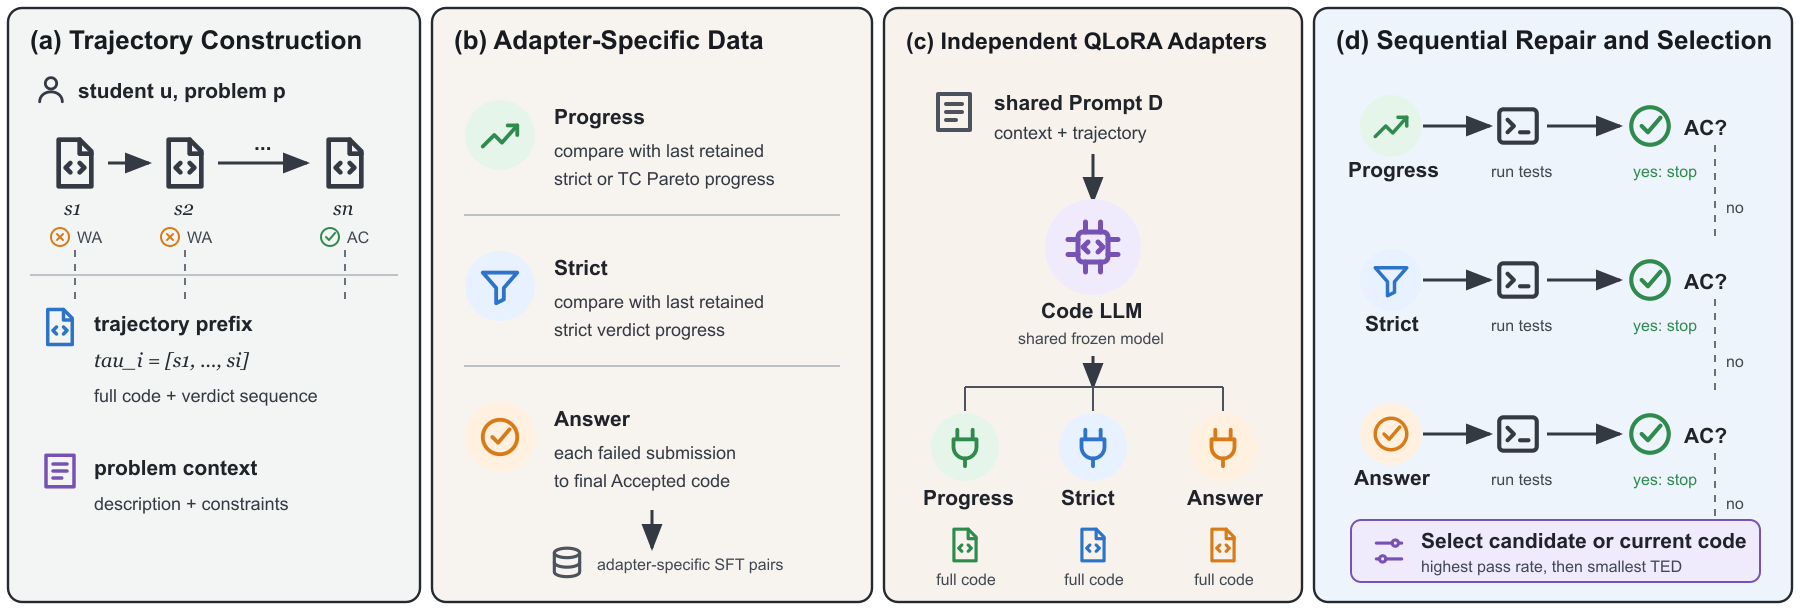
\includegraphics[width=\linewidth]{Figures/zpdpatch_overview_v4.png}
  \caption{Overview of \tool. Authentic submission trajectories are normalized and re-executed. Adapter-specific rules construct supervision for \progress, \strict, and \answer. Independently trained adapters generate candidates sequentially; execution outcomes determine early stopping and final selection.}
  \Description{The ZPDPatch pipeline converts student submission trajectories and cached test outcomes into Progress, Strict, and Answer training pairs. At inference time, the three adapters generate repair candidates in sequence, with execution-based early stopping and final candidate selection.}
  \label{fig:overview}
\end{figure}

\subsection{Design Requirements}

The method is organized around four requirements derived from the deployment setting. \emph{Automatic supervision} requires every target to be recoverable from submissions, verdicts, and tests, without a teacher labeling which edit is pedagogically appropriate. \emph{Target diversity} requires the training construction to expose both intermediate improvements and complete solutions; otherwise, one model objective must conflate conservative and answer-level repair. \emph{Executable validation} requires generated programs to be judged by the same external runner rather than by model confidence or textual similarity. Finally, \emph{non-regression} requires the system to retain the current program whenever no generated candidate improves its executed behavior.

These requirements lead to a separation between offline and online decisions. Offline, one trajectory can yield multiple supervised examples under different policies. Online, each policy proposes at most one candidate, but execution decides whether the candidate should terminate the sequence, inform the next stage, or be ignored by the final selector. This separation is important: the label rules define what a model learns, whereas the selector defines what the deployed system is permitted to return. A noisy training transition can influence generation without automatically overriding a better current program.

\subsection{Trajectory Construction}

We group submissions by problem and student, sort them by timestamp, and terminate at the first \texttt{Accepted} submission. We normalize indentation, remove comments and blank lines, and remove consecutive submissions that are identical after normalization. Until adapter-specific filtering, we preserve complete source code, original verdict, order, and all observed history. We impose no maximum history length or transition count. We also re-execute every submission on the available tests and cache per-test outcomes for deterministic reuse in dataset construction and evaluation.

Termination at the first acceptance prevents a solved problem from contributing post-solution experimentation as if it were part of the repair path. Consecutive duplicate removal avoids overweighting resubmissions that differ only in comments or formatting. We do not deduplicate non-consecutive states because returning to an earlier program is itself part of the observed trajectory and may separate two distinct attempts. Normalization is used only for duplicate detection; the model input and target preserve complete normalized source rather than an edit script.

The execution cache binds an outcome to the tuple of problem, normalized code, test-suite identity, timeout, and memory limit. This key prevents reuse across incompatible execution settings. Failed runner invocations are represented explicitly and receive the most severe internal outcome; they are not silently treated as wrong answers. Adapter construction reads only completed cache entries, making the same per-test evidence available to dataset creation, stage feedback, and evaluation.

\subsection{Adapter-Specific Supervision}
\label{sec:supervision}

We order verdict severity as
\(\mathrm{sev}(\texttt{AC})=0\),
\(\mathrm{sev}(\texttt{WA})=1\),
\(\mathrm{sev}(\texttt{TLE/MLE})=2\),
\(\mathrm{sev}(\texttt{RE})=3\),
\(\mathrm{sev}(\texttt{CE})=4\),
and 5 for internal failures. For equal, non-empty test keys, \(o_t\preceq_{\mathrm{sev}}o_r\) iff no test outcome in \(o_t\) is more severe than its counterpart in \(o_r\). Test-case progress is the Pareto condition
\begin{equation}
\mathrm{TCProg}(r,t)=
\mathbf{1}\!\left[o_t\preceq_{\mathrm{sev}}o_r \land o_t\neq o_r\right].
\label{eq:tcprogress}
\end{equation}

\paragraph{Answer.}
If \(s_n\) is accepted, every preceding non-accepted submission is independently paired with \(c_n\). For \(\tau=[S_1,\ldots,S_9]\), the rule produces \(([S_1],c_9),\ldots,([S_8],c_9)\). Thus, \answer learns a direct failed-program-to-answer mapping and receives no multi-submission history.

\paragraph{Strict.}
Starting with \(R=[s_1]\), we scan the trajectory and append \(s_t\) only when its verdict is strictly better than the last retained submission \(s_r=R[-1]\): \(\mathrm{sev}(v_t)<\mathrm{sev}(v_r)\). If \(R=[r_1,\ldots,r_m]\), we create \(([r_1,\ldots,r_{k-1}],c_{r_k})\) for every \(k=2,\ldots,m\). The comparison is against the last retained state, not necessarily the immediately preceding original submission.

\paragraph{Progress.}
\progress uses the same retained scan but appends \(s_t\) when either its verdict strictly improves or \(v_t=v_r\) and \(\mathrm{TCProg}(r,t)=1\). It therefore captures monotonic per-test progress that is hidden by an unchanged coarse verdict. Prefix-target construction is otherwise identical to \strict.

The datasets are constructed independently and may overlap. A strict transition is also a progress transition, and final accepted transitions can occur in both. The objectives nevertheless differ: \answer learns direct completion from one failed program, whereas \strict and \progress learn transitions from retained prefixes.

Algorithm~\ref{alg:construct} gives the common retained-prefix construction. The predicate \textsc{Keep} is the only difference between \strict and \progress. Comparing a candidate with the last retained state, rather than the immediately previous raw submission, makes the retained sequence monotonic under the selected rule. Importantly, the algorithm emits every retained prefix. A trajectory with \(m\) retained states yields \(m-1\) training examples, so early transitions are not discarded in favor of only the final prefix.

\begin{algorithm}[t]
\caption{Retained-prefix supervision for \strict and \progress}
\label{alg:construct}
\begin{algorithmic}[1]
\Require Trajectory \(\tau=[s_1,\ldots,s_n]\), policy \(a\in\{\mathrm{strict},\mathrm{prog}\}\)
\Ensure Supervised examples \(D_a\)
\State \(R\gets[s_1]\); \(D_a\gets[]\)
\For{\(t\gets2\) to \(n\)}
  \State \(r\gets R[-1]\)
  \State \(q\gets \mathrm{sev}(v_t)<\mathrm{sev}(v_r)\)
  \If{\(a=\mathrm{prog}\)}
    \State \(q\gets q\lor(v_t=v_r\land\mathrm{TCProg}(r,t))\)
  \EndIf
  \If{\(q\)}
    \State append \((R,c_t)\) to \(D_a\); append \(s_t\) to \(R\)
  \EndIf
\EndFor
\State \Return \(D_a\)
\end{algorithmic}
\end{algorithm}

\subsection{Illustrative Trajectory}

Consider an illustrative trajectory with verdicts
\[
[\texttt{RE},\texttt{WA},\texttt{WA},\texttt{WA},\texttt{AC}]
\]
and three-test outcome vectors
\[
[(\texttt{RE},\texttt{RE},\texttt{RE}),
 (\texttt{AC},\texttt{WA},\texttt{WA}),
 (\texttt{AC},\texttt{AC},\texttt{WA}),
 (\texttt{AC},\texttt{WA},\texttt{WA}),
 (\texttt{AC},\texttt{AC},\texttt{AC})].
\]
The example is synthetic and serves only to clarify the rules. \strict retains \(S_1,S_2,S_5\): the transition from runtime error to wrong answer improves verdict severity, the two later wrong-answer states do not, and acceptance improves again. It emits \(([S_1],c_2)\) and \(([S_1,S_2],c_5)\).

\progress additionally retains \(S_3\), because one test changes from wrong answer to accepted while no test regresses relative to \(S_2\). It rejects \(S_4\): relative to the last retained state \(S_3\), the second test regresses from accepted to wrong answer. The retained sequence is therefore \(S_1,S_2,S_3,S_5\), yielding three prefix-target examples. \answer ignores these intermediate relations and emits four independent pairs \(([S_1],c_5),\ldots,([S_4],c_5)\). This example exposes three consequences of the design. Progress is monotonic with respect to observed per-test outcomes, Strict can skip locally useful same-verdict edits, and Answer can learn from a failed state even when that state would be removed by both retained scans.

The construction does not assume that the student's next raw submission is a desirable target. A later submission can revert a passing test, introduce a compilation error, or repeat an earlier program. Such states remain part of the authentic record but do not become \progress or \strict targets unless they satisfy the corresponding comparison. Conversely, a non-adjacent later state may become the target when intervening submissions fail the rule. The objective is thus filtered transition learning, not next-submission imitation.

\subsection{Prompt and Adapter Training}

All adapters use the same prompt. The system message contains the problem statement and resource limits. Each retained submission is represented by its complete code and online verdict; cached per-test outcomes and an AST/line edit summary are included when available. The final user message is the current program and the assistant target is one complete Python program. The prompt never names an adapter role, so specialization can arise only from supervision.

The serialized prompt has three layers. The problem layer fixes the natural-language specification and resource limits for every example of a problem. The history layer presents retained submissions chronologically and identifies their observed verdicts; when more than one submission is present, structural and line-level summaries describe the intervening change without replacing either full program. The query layer repeats the current state and requests exactly one complete Python program. We avoid a role instruction such as ``make a small change'' or ``provide the answer,'' because that wording would confound supervision with prompt engineering in the adapter comparison.

Only assistant target tokens contribute to the loss. This mask prevents long statements or histories from dominating the objective merely because they contain more tokens. Whole-program targets also avoid a separate patch-application failure mode: every decoded candidate can be written to a file and executed directly. The cost is that even a one-line semantic change requires generating the complete program, which motivates greedy decoding and early stopping in the online sequence.

For adapter \(a\in\{\mathrm{prog},\mathrm{strict},\mathrm{ans}\}\), let \(\mathcal{D}_a\) be its dataset, \(x_i\) the prompt, and \(y_i\) the target tokens. We minimize the target-only supervised fine-tuning objective
\begin{equation}
\mathcal{L}_a=-\frac{1}{|\mathcal{D}_a|}
\sum_{(x_i,y_i)\in\mathcal{D}_a}
\frac{1}{|y_i|}\sum_{k=1}^{|y_i|}
\log P_{\theta,\phi_a}(y_{i,k}\mid y_{i,<k},x_i),
\label{eq:sft}
\end{equation}
where \(\theta\) is the frozen base model and \(\phi_a\) is an adapter's QLoRA parameter set. Prompt tokens are masked from the loss. The adapters are trained and stored independently.

\subsection{Execution-Guided Sequential Repair}
\label{sec:sequential}

At inference time, we execute the observed submissions to populate consistent feedback and then invoke \progress, \strict, and \answer in that order. Each adapter generates one complete program. A candidate that passes every test is returned immediately. Otherwise, its verdict, pass rate, per-test outcomes, and improvement status are appended to the next-stage prompt. For a no-op or regression, only the execution result is passed forward, avoiding reinforcement of the candidate code.

The order is fixed before evaluation. \progress is first because its training targets admit fine-grained, non-regressive test improvements; \strict follows with a coarser verdict-improvement objective; \answer is last because its direct accepted targets permit the broadest change. This ordering is a design prior rather than a claim that one adapter is intrinsically easier. RQ3 evaluates the adapters independently, and RQ4 tests whether their fixed composition adds value beyond each member.

If all candidates fail, the selector includes the current program \(c_i\) as a fallback:
\begin{equation}
\mathcal{C}=\{c_i,c^{\mathrm{prog}},c^{\mathrm{strict}},c^{\mathrm{ans}}\}.
\end{equation}
Let \(\mathrm{Pass}(c)\) be the fraction of tests passed and \(\mathrm{ted}(c_i,c)\) the Python AST tree edit distance. Selection is lexicographic:
\begin{equation}
c^*=\underset{c\in\mathcal{C}}{\arg\max}
\left(\mathrm{Pass}(c),-\mathrm{ted}(c_i,c)\right).
\label{eq:selection}
\end{equation}
The selector first maximizes executed correctness and then minimizes change. If no candidate improves on \(c_i\), the unchanged fallback has TED zero and the system abstains.

Algorithm~\ref{alg:repair} makes the information flow explicit. The working context is not identical to the original student trajectory after the first stage: it may contain generated execution feedback. However, generated code is included only when it improves the current pass rate. This rule avoids presenting a regressive program to the next adapter as if it were a student-authored advance. Every generated candidate remains in the selector pool, where executed correctness dominates edit distance.

\begin{algorithm}[t]
\caption{Execution-guided sequential repair}
\label{alg:repair}
\begin{algorithmic}[1]
\Require Problem \(p\), current code \(c_i\), observed context \(h\)
\State \(C\gets[c_i]\); \(q_0\gets\mathrm{Pass}(c_i)\); \(H\gets h\)
\For{\(a\) in \([\mathrm{Progress},\mathrm{Strict},\mathrm{Answer}]\)}
  \State \(c^a\gets\mathrm{Generate}(a,p,H)\)
  \State \(z^a\gets\mathrm{Execute}(p,c^a)\); append \(c^a\) to \(C\)
  \If{\(\mathrm{Pass}(c^a)=1\)}
    \State \Return \(c^a\)
  \ElsIf{\(\mathrm{Pass}(c^a)>q_0\)}
    \State append \((c^a,z^a)\) to \(H\)
  \Else
    \State append \(z^a\) to \(H\)
  \EndIf
\EndFor
\State \Return \(\arg\max_{c\in C}(\mathrm{Pass}(c),-\mathrm{ted}(c_i,c))\)
\end{algorithmic}
\end{algorithm}

\subsection{Properties and Computational Cost}

Two properties follow directly from the construction. First, the retained sequences for \strict and \progress are monotonic under their own predicates. This does not imply monotonic source-code similarity: a student can make a large rewrite while improving one verdict. Second, final selection is non-regressive on the observed test suite because \(c_i\in\mathcal C\) and pass rate is the primary key. If every candidate has a lower pass rate, \(c_i\) wins; if candidates tie its pass rate, its zero self-distance wins the secondary key unless a generated program is structurally identical.

For a raw trajectory of length \(n\) and \(T\) tests, dataset construction performs a single retained scan once cached outcomes exist. Comparing outcome vectors costs \(O(T)\), giving \(O(nT)\) time and \(O(n)\) retained-state storage per trajectory, excluding program text. Answer construction is \(O(n)\). At inference, generation dominates cost. The system performs between one and three generations and executions, with exactly three only when neither early stage produces an accepted program. The cache can eliminate repeated execution for identical candidates but does not change the worst-case generation count.

\section{Experimental Design}
\label{sec:experiment}

\subsection{Research Questions}

\begin{description}
  \item[RQ1: Repair Effectiveness.] How effectively does \tool repair held-out trajectories from problems observed during training, compared with zero-shot and retrieval-based repair?
  \item[RQ2: Trajectory Conditioning.] Does access to the full submission prefix improve repair over training and inference with only the current code?
  \item[RQ3: Adapter Specialization.] Do \progress, \strict, and \answer exhibit different repair coverage and patch size?
  \item[RQ4: Sequential Escalation.] Does execution-guided composition improve effectiveness without always invoking all adapters?
  \item[RQ5: Problem Generalization.] Does \tool retain an advantage on problems completely excluded from training?
\end{description}

\subsection{Dataset Construction and Splits}

We combine Python submissions, statements, metadata, and test cases for problems in Project CodeNet's Python800 benchmark~\cite{puri2021project}. We retain trajectories with at least three submissions, at least one non-accepted state before the first acceptance, and a final accepted program present in the Python800 reference set. We remove post-acceptance submissions and consecutive normalized duplicates. Users must appear in at least three problems and each retained problem must contain at least two trajectories. The refined corpus contains 546 problems, 21,454 trajectories, 99,432 submissions, and 10,088 tests.

Before splitting, we tokenize every possible \answer, \strict, conservative \progress, and final-evaluation prompt-target configuration. If any configuration exceeds 4,096 tokens, we exclude the entire trajectory rather than truncating code or history. This removes 2,896 trajectories and leaves 18,558. No later \texttt{max\_history}, transition-count, code, or test truncation is applied.

We sort problems by eligible trajectory count and assign the top 90\% (492 problems) to \emph{Seen} and the remaining 54 low-resource problems to \emph{Unseen}. Within every Seen problem, we reserve at least one trajectory for Train, Validation, and Test, then obtain a deterministic 80:10:10 trajectory split. All 260 Unseen trajectories remain problem-held-out test data. Table~\ref{tab:data} reports the resulting corpus. Users may occur in more than one split; RQ5 is problem-held-out, not user-held-out.

\begin{table}[t]
\caption{Dataset statistics after whole-trajectory context filtering. ``Prefix'' counts possible raw prefixes before adapter-specific filtering.}
\label{tab:data}
\centering
\small
\begin{tabular}{llrrrrrr}
\toprule
Group & Role & Problems & Tests & Traj. & Sub. & Prefix & Users \\
\midrule
\multirow{3}{*}{Seen}
 & Train & \multirow{3}{*}{492} & \multirow{3}{*}{9,446} & 14,638 & 58,872 & 44,234 & 4,072 \\
 & Validation & & & 1,830 & 7,283 & 5,453 & 1,283 \\
 & Test & & & 1,830 & 7,068 & 5,238 & 1,291 \\
\midrule
Unseen & Test & 54 & 642 & 260 & 965 & 705 & 237 \\
\bottomrule
\end{tabular}
\end{table}

Adapter construction yields the training and validation sizes in Table~\ref{tab:adapter-data}. Final evaluation uses the prefix ending at the last non-accepted submission and the final accepted program as the oracle. We retain only cases for which re-execution confirms the current program as non-accepted and the oracle as accepted, leaving 997 Seen and 250 Unseen repair instances.

\begin{table}[t]
\caption{Adapter supervision datasets. Validation examples are excluded from training.}
\label{tab:adapter-data}
\centering
\begin{tabular}{lrr}
\toprule
Adapter & Train examples & Validation examples \\
\midrule
\progress & 21,416 & 2,685 \\
\strict & 16,973 & 2,116 \\
\answer & 40,454 & 4,965 \\
\bottomrule
\end{tabular}
\end{table}

\subsection{Baselines}

\paragraph{Zero-shot.}
The zero-shot baseline uses the same Qwen base model and prompt as \tool without fine-tuning. If a candidate fails, its verdict and number of passed tests are added to the conversation before the next attempt. It receives at most three generations, matching \tool's maximum budget. Because it receives the full trajectory, comparison with zero-shot measures the complete effect of learned adapters and sequential composition, not history in isolation.

\paragraph{LSGen.}
LSGen is an iterative retrieval-based solution generator~\cite{dai2026learner}. We preserve its repair-pair filtering, edit-vector retrieval, diff-guided generation, and re-retrieval, while replacing hard-coded infrastructure with our common dataset and runner. For a Seen query, the retrieval database contains buggy/correct pairs from other Seen-Train trajectories of the same problem; the same student and example are excluded. LSGen retrieves five pairs and performs at most three iterations. We do not evaluate it on Unseen problems because exposing same-problem correct programs would violate problem holdout.

All approaches use the same base LLM, public tests, 2.5-second per-test timeout, 2GB memory limit, and maximum of three candidate generations.

\subsection{Implementation}

We use Qwen2.5-Coder-7B-Instruct~\cite{hui2024qwen2} and train each adapter for one epoch with 4-bit QLoRA~\cite{dettmers2023qlora}. The base weights use NF4 double quantization and BF16 computation. LoRA targets the \(q,k,v,o\) attention projections and gate/up/down MLP projections with rank 16, scaling 32, and dropout 0.05. Optimization uses paged 8-bit AdamW, learning rate \(2\times10^{-4}\), cosine scheduling, 0.03 warmup ratio, gradient checkpointing, micro-batches of 2, eight accumulation steps, and seed 2027. We select the lowest validation-loss checkpoint. Greedy decoding uses all model context remaining after the input. Training and generation run on one NVIDIA RTX 5090.

A single Python runner executes original and generated programs. We cache outcomes by problem, code, test set, timeout, and memory configuration and reuse the cache across supervision construction, stage feedback, and evaluation. Candidate generation can proceed in parallel, but candidate execution and recorded outcomes are shared so that an identical program cannot receive inconsistent labels under CPU contention.

\subsection{Ablations}

For RQ2, we construct adapter-specific \strict and \progress examples for both Seen and Unseen tests. \emph{Full Trajectory} uses each retained prefix. \emph{Current Code Only} retrains an adapter on identical examples and targets after removing every submission before the current one; its displayed position is reset to \(S_1\) to prevent index leakage. \answer is excluded because its inputs already contain one submission. This design isolates the presence of history while holding targets, counts, model, and hyperparameters fixed.

For RQ3, each adapter independently generates one candidate for the same 997 Seen instances. For RQ4, we compare these individual candidates with the full \progress--\strict--\answer sequence, including stage feedback, early stopping, and fallback selection.

\subsection{Metrics and Statistical Analysis}

For \(M\) instances, let \(c_m\) be the current program and \(\hat c_m\) the selected result. \(\mathrm{Pass}(c)\in[0,1]\) is the test pass fraction. Pass Rate (PR) averages \(\mathrm{Pass}(\hat c_m)\); Repair Rate (RR) averages \(\mathbf{1}[\mathrm{Pass}(\hat c_m)=1]\); Improvement Rate (IR) averages \(\mathbf{1}[\mathrm{Pass}(\hat c_m)>\mathrm{Pass}(c_m)]\).

Average Time Taken (ATT) is weighted wall-clock time per repaired input, measured from generation through execution and selection for all inputs of a problem. Shared cache construction, model loading, training, and LSGen database construction are offline preparation and excluded.

For successfully repaired, parseable programs, \(\mathrm{TED}_{B\rightarrow F}\) measures AST distance from current to fixed code and \(\mathrm{TED}_{F\rightarrow O}\) from fixed code to the recorded accepted oracle. RQ2 uses \(\mathrm{TED}_{F\rightarrow T}\), where \(T\) is the identical adapter-specific recorded target shared by Full and Current configurations.

We report Wilson 95\% intervals for RR and IR. Paired RR comparisons use two-sided exact McNemar tests. Paired PR and TED differences use 10,000 bootstrap resamples with seed 2027. We apply Holm correction within each planned family of RR comparisons: the three RQ1 methods, four RQ2 adapter-split comparisons, three RQ3 adapter comparisons, and three RQ4 comparisons against Sequential. Unless stated otherwise, percentages are absolute percentage points.

\section{Results}
\label{sec:results}

\subsection{RQ1: Repair Effectiveness}

Table~\ref{tab:main-results} summarizes RQ1 and RQ5. On Seen problems, \tool repairs 564 of 997 programs (56.6\%), compared with 306 (30.7\%) for Zero-shot. Their Wilson RR intervals are [53.5, 59.6] and [27.9, 33.6], respectively. \tool alone repairs 301 instances, whereas Zero-shot alone repairs 43 (Holm-adjusted McNemar \(p=1.64\times10^{-48}\)). PR increases by 8.57 points (95\% bootstrap CI [6.99, 10.22]) and IR by 20.9 points.

LSGen achieves the highest Seen execution correctness: 88.0\% PR, 80.2\% RR, and 82.4\% IR. It alone repairs 306 instances, while \tool alone repairs 70 (Holm-adjusted \(p=2.70\times10^{-36}\)). The tradeoff is patch size. \tool's mean \(\mathrm{TED}_{B\rightarrow F}\) is 19.71, versus 27.25 for Zero-shot and 88.27 for LSGen. Among jointly repaired parseable instances, \tool reduces TED by 8.07 relative to Zero-shot (95\% CI [4.53, 12.14]) and by 43.41 relative to LSGen (95\% CI [38.20, 48.94]). \tool also has the lowest Seen ATT at 12.16 seconds, though timing differences are small.

\begin{table}[t]
\caption{Main repair results. PR, RR, and IR are percentages; ATT is seconds. TED is computed on successfully repaired, parseable programs.}
\label{tab:main-results}
\centering
\small
\begin{tabular}{llrrrrrr}
\toprule
Split & Method & PR & RR & IR & ATT & \(\mathrm{TED}_{B\to F}\) & \(\mathrm{TED}_{F\to O}\) \\
\midrule
\multirow{3}{*}{Seen}
 & Zero-shot & 76.3 & 30.7 & 43.7 & 12.87 & 27.25 & 27.67 \\
 & LSGen & \textbf{88.0} & \textbf{80.2} & \textbf{82.4} & 13.00 & 88.27 & 83.23 \\
 & \tool & 84.9 & 56.6 & 64.6 & \textbf{12.16} & \textbf{19.71} & \textbf{21.89} \\
\midrule
\multirow{2}{*}{Unseen}
 & Zero-shot & 75.3 & 62.0 & 68.8 & \textbf{3.89} & 17.46 & 15.80 \\
 & \tool & \textbf{83.0} & \textbf{72.0} & \textbf{76.8} & 6.17 & \textbf{11.66} & \textbf{12.54} \\
\bottomrule
\end{tabular}
\end{table}

The aggregate rates conceal how often two methods repair the same inputs. Table~\ref{tab:paired-outcomes} reconstructs the paired outcome counts used by the McNemar comparisons. Against Zero-shot on Seen data, the two methods jointly repair 263 inputs, but \tool repairs 301 additional inputs that Zero-shot misses; the reverse occurs for 43. Thus, the system-level gain is not merely a small set of exchanged successes. Against LSGen, the overlap is much larger: both repair 494 inputs. LSGen nevertheless repairs 306 inputs that \tool misses, while the learned system uniquely repairs 70. This pattern explains why LSGen has higher RR while neither method's success set strictly contains the other.

\begin{table}[t]
\caption{Paired complete-repair outcomes. ``Only \tool'' and ``only comparator'' are the discordant pairs used by McNemar tests. Counts are derived from the same instances as Table~\ref{tab:main-results}.}
\label{tab:paired-outcomes}
\centering
\small
\begin{tabular}{llrrrr}
\toprule
Split & Comparator & Both & Only \tool & Only comparator & Neither \\
\midrule
Seen & Zero-shot & 263 & 301 & 43 & 390 \\
Seen & LSGen & 494 & 70 & 306 & 127 \\
Unseen & Zero-shot & 138 & 42 & 17 & 53 \\
\bottomrule
\end{tabular}
\end{table}

PR and IR add information beyond complete repair. On Seen data, the 25.9-point RR gain over Zero-shot is accompanied by an 8.6-point PR gain and a 20.9-point IR gain. The smaller PR difference is expected because PR gives partial credit to failed programs that pass some tests. In other words, Zero-shot often produces behavior that is partly correct without reaching acceptance, whereas \tool converts more of those opportunities into full repairs. The selector's unchanged fallback also affects IR: an abstention is not an improvement, but it avoids counting a regression as progress.

Patch distance separates effectiveness from replacement. \tool's mean current-to-fix TED is 27.7\% lower than Zero-shot's and 77.7\% lower than LSGen's among the respective successful sets. These unpaired percentage summaries should not be interpreted as statistical comparisons because each mean is computed on a different success subset; the paired bootstrap results reported above are the primary evidence. Both paired comparisons point in the same direction, showing that the conclusion is not only an artifact of which instances each method repairs.

\paragraph{Answer to RQ1.}
\tool substantially outperforms a trajectory-prompted zero-shot model and produces smaller successful patches. Same-problem retrieval remains much stronger in repair coverage, so \tool is complementary to, rather than a replacement for, a correct-solution database.

\subsection{RQ2: Trajectory Conditioning}

Table~\ref{tab:rq2} shows no consistent advantage for Full Trajectory. On Seen \strict examples, Full raises PR by 0.7 points but lowers RR and IR by 0.7 and 1.3. On Seen \progress, it lowers PR, RR, and IR by 1.0, 0.4, and 0.6. On Unseen data, Full is worse for \strict but better for \progress. Target TED is also mixed: Full is closer to the recorded target for Seen \progress and Unseen \strict, but farther in the other conditions. None of the four paired RR differences is significant after Holm correction (minimum adjusted \(p=0.313\)).

\begin{table}[t]
\caption{RQ2 trajectory-conditioning results. PR, RR, and IR are percentages. Current and Full use identical examples and targets.}
\label{tab:rq2}
\centering
\small
\begin{tabular}{lllrrrrr}
\toprule
Split & Adapter & Input & \(N\) & PR & RR & IR & \(\mathrm{TED}_{F\to T}\) \\
\midrule
\multirow{4}{*}{Seen}
 & \strict & Current & 2,151 & 56.8 & 31.2 & 54.6 & 40.23 \\
 & \strict & Full & 2,151 & 57.5 & 30.5 & 53.3 & 41.05 \\
 & \progress & Current & 2,674 & 58.4 & 26.3 & 49.7 & 36.23 \\
 & \progress & Full & 2,674 & 57.4 & 25.9 & 49.1 & 33.15 \\
\midrule
\multirow{4}{*}{Unseen}
 & \strict & Current & 322 & 66.7 & 56.2 & 71.4 & 20.20 \\
 & \strict & Full & 322 & 65.4 & 53.4 & 70.8 & 19.27 \\
 & \progress & Current & 378 & 65.7 & 52.1 & 66.4 & 17.63 \\
 & \progress & Full & 378 & 66.5 & 53.7 & 68.3 & 18.16 \\
\bottomrule
\end{tabular}
\end{table}

The ablation is paired at three levels. Within each row pair, the training example identities and target programs are identical. The same adapter architecture and hyperparameters are used, and evaluation compares the two models on the same inputs. The only intended change is whether submissions before the current program are serialized in the prompt. This design prevents a larger Full dataset or a different target distribution from masquerading as a history effect.

The direction changes across all four conditions. Full loses 0.7 RR points for Seen \strict and 0.4 for Seen \progress; it loses 2.8 points for Unseen \strict but gains 1.6 for Unseen \progress. The absolute differences are small relative to the variation in baseline difficulty between Seen and Unseen rows, and no corrected comparison is significant. TED does not rescue a consistent history claim: the history-conditioned model is closer to its target in two conditions and farther in two. Thus, neither execution success nor imitation of the recorded target supplies a stable directional result.

This null result is informative because the zero-shot and full-system prompts still contain trajectory context. RQ1 asks whether the complete learned and sequential method is useful in that operating configuration. RQ2 asks the narrower causal question of whether retaining earlier submissions improves an otherwise matched adapter. The first answer can be positive while the second is negative. Keeping these estimands separate prevents the complete system's improvement from being attributed to a component that the controlled ablation does not support.

\paragraph{Answer to RQ2.}
Providing full submission history does not consistently improve repair over current code alone. RQ1 therefore cannot be interpreted as evidence for a causal history-conditioning effect; it measures the complete learned and sequential system.

\subsection{RQ3: Adapter Specialization}

Table~\ref{tab:rq3} exposes a coverage-size tradeoff. \answer has the highest PR, RR, and IR, but also the largest mean patch at TED 20.22. \progress has lower coverage but the smallest patch at TED 15.85. \strict and \progress have statistically indistinguishable RR (adjusted \(p=0.857\)). \answer repairs 5.2 points more than \progress and 5.5 points more than \strict (adjusted \(p=6.21\times10^{-4}\) and \(1.92\times10^{-4}\), respectively). The ordered increase in patch size is consistent with broader targets, but \strict does not form a clearly distinct coverage regime.

\begin{table}[t]
\caption{RQ3 individual-adapter results on 997 Seen instances.}
\label{tab:rq3}
\centering
\begin{tabular}{lrrrrr}
\toprule
Adapter & PR & RR & IR & \(\mathrm{TED}_{B\to F}\) & \(\mathrm{TED}_{F\to O}\) \\
\midrule
\progress & 73.4 & 44.8 & 52.0 & \textbf{15.85} & \textbf{15.89} \\
\strict & 74.8 & 44.5 & 51.2 & 17.45 & 18.38 \\
\answer & \textbf{77.5} & \textbf{50.1} & \textbf{57.5} & 20.22 & 20.61 \\
\bottomrule
\end{tabular}
\end{table}

The individual results reveal two distinct notions of specialization. \emph{Coverage specialization} is weak between \progress and \strict: their RR differs by only 0.3 points, and the corrected paired comparison is not significant. \emph{Patch-scope specialization} is clearer. Strict increases current-to-fix TED from 15.85 to 17.45, and Answer increases it to 20.22. Relative to Progress, Answer's successful patches are 27.6\% larger by mean TED while repairing 5.3 percentage points more inputs. The supervision rules therefore order modification size more clearly than they order complete-repair coverage.

Distance to the recorded accepted oracle follows the same pattern. Progress has the lowest mean \(\mathrm{TED}_{F\to O}\) at 15.89, Strict reaches 18.38, and Answer reaches 20.61. This does not mean that Progress copies the oracle: its targets can be intermediate non-accepted programs, and the metric is computed only when its generated candidate is accepted. Rather, on the subset it repairs, Progress tends to reach an accepted program through a smaller structural move from both the current state and the recorded oracle. Answer covers more cases at the cost of broader edits.

These averages also caution against interpreting adapter names as guaranteed behaviors on every input. An Answer candidate can be small, and a Progress candidate can rewrite a program. The rules shape training distributions, not hard constraints at decoding time. Hard non-regression and minimum-edit preferences enter only through execution and final selection.

\paragraph{Answer to RQ3.}
The supervision rules induce different repair-size behavior: direct answer supervision produces the broadest and most successful individual adapter, while progress supervision produces the smallest successful patches. Verdict-only \strict is not clearly separated from \progress in repair coverage.

\subsection{RQ4: Sequential Escalation}

Sequential repair reaches 56.6\% RR, 6.5 points above the strongest individual adapter, \answer. Sequential alone repairs 119 cases and \answer alone repairs 54 (Holm-adjusted \(p=8.57\times10^{-7}\)). Its advantage over \progress and \strict is also significant (adjusted \(p=1.64\times10^{-22}\) and \(1.87\times10^{-21}\)).

Early stopping limits cost. Of 997 inputs, 439 stop after \progress and another 66 after \strict. The system generates 2.05 candidates on average instead of always generating three. ATT is 12.16 seconds, only 2.17 seconds above the fastest individual adapter. The final selector returns a \progress candidate for 484 instances, \strict for 88, \answer for 72, and the unchanged fallback for 353.

Table~\ref{tab:stage-flow} expands this control flow. Every input reaches Progress. The 439 accepted Progress candidates terminate immediately, so 558 inputs reach Strict. Strict accepts 66 more, leaving 492 inputs for Answer. The resulting number of generations is \(997+558+492=2{,}047\), or 2.05 per input. Always invoking all adapters would require 2,991 generations; early stopping therefore avoids 944 generations, 31.6\% of the fixed three-stage budget.

\begin{table}[t]
\caption{RQ4 stage flow and final selector provenance on 997 Seen inputs. ``Reached'' counts generated candidates; ``accepted here'' counts early stops. Selector provenance includes early stops and final selection.}
\label{tab:stage-flow}
\centering
\small
\begin{tabular}{lrrr}
\toprule
Stage / source & Reached & Accepted here & Returned by system \\
\midrule
\progress & 997 & 439 & 484 \\
\strict & 558 & 66 & 88 \\
\answer & 492 & -- & 72 \\
Unchanged fallback & -- & -- & 353 \\
\bottomrule
\end{tabular}
\end{table}

The returned-source counts differ from the early-stop counts because selection can recover a non-accepted earlier candidate after all stages fail. Progress is returned 484 times, 45 more than its immediate acceptances, and Strict is returned 88 times, 22 more than its immediate acceptances. Answer is returned 72 times after the final comparison. The unchanged program is returned for 353 inputs, making abstention a substantial part of system behavior rather than a corner case. Of these fallback returns, the table alone does not distinguish ties from cases where every candidate regressed, so we do not assign a more specific failure interpretation.

\begin{table}[t]
\caption{RQ4 sequential escalation on 997 Seen instances. ``Candidates'' is the mean number generated.}
\label{tab:rq4}
\centering
\begin{tabular}{lrrrrr}
\toprule
Configuration & PR & RR & IR & ATT & Candidates \\
\midrule
\progress & 73.4 & 44.8 & 52.0 & 10.91 & 1.00 \\
\strict & 74.8 & 44.5 & 51.2 & 10.95 & 1.00 \\
\answer & 77.5 & 50.1 & 57.5 & \textbf{9.99} & 1.00 \\
Sequential & \textbf{84.9} & \textbf{56.6} & \textbf{64.6} & 12.16 & 2.05 \\
\bottomrule
\end{tabular}
\end{table}

\paragraph{Answer to RQ4.}
Execution-guided escalation improves both complete repair and partial improvement over every single adapter. Early stopping avoids a fixed three-generation cost, although the sequence still averages roughly twice the generation work of an individual adapter.

\subsection{RQ5: Problem Generalization}

On 250 Unseen instances, \tool obtains 83.0\% PR, 72.0\% RR, and 76.8\% IR, versus 75.3\%, 62.0\%, and 68.8\% for Zero-shot. \tool alone repairs 42 cases and Zero-shot alone repairs 17 (McNemar \(p=0.00155\)). The PR difference is 7.65 points (95\% bootstrap CI [3.59, 11.93]). \tool also reduces mean successful-patch TED from 17.46 to 11.66. Among joint repairs, its patch is 6.33 TED units smaller on average (95\% CI [3.31, 9.77]).

The Unseen contingency in Table~\ref{tab:paired-outcomes} shows 138 joint repairs, 42 unique \tool repairs, 17 unique Zero-shot repairs, and 53 failures by both. The 10-point RR advantage is therefore supported by more than twice as many favorable as unfavorable discordant pairs. At the same time, 17 Zero-shot-only successes show that fine-tuning and sequential selection do not dominate the base model on every held-out problem. A portfolio that could recognize these complementary successes without test leakage remains a possible extension.

The absolute Unseen RR is higher for both systems than their Seen RR. This cannot be read as a conventional train--test generalization comparison because the groups were created by problem trajectory count, not randomized by difficulty. The Unseen group contains lower-resource problems and a different mixture of statements, tests, and current-program states. The defensible comparison is within Unseen: both methods face the same 250 instances, and \tool retains a paired advantage without same-problem adapter training.

\paragraph{Answer to RQ5.}
\tool's advantage over Zero-shot persists on problems completely excluded from adapter training. Because the Unseen group deliberately contains lower-resource problems, its higher absolute RR must not be interpreted as evidence that unseen problems are easier or that familiarity harms repair.

\subsection{Cross-RQ Synthesis}

The five questions support a layered account of the system. RQ1 establishes that the complete method improves substantially over a trajectory-prompted base model, while also documenting a coverage deficit relative to same-problem retrieval. RQ2 removes a tempting explanation for that gain: earlier submissions in the prompt do not provide a consistent benefit under matched training targets. RQ3 shows that changing the trajectory-derived target rule changes patch scope more reliably than repair coverage. RQ4 then demonstrates that execution-guided composition recovers additional repairs beyond the strongest individual adapter. RQ5 shows that the learned system's advantage over Zero-shot persists when problem identities are held out.

Taken together, the results locate the strongest evidence in two components. First, authentic trajectories are useful as an offline source of diverse repair transitions. Second, executed outcomes are useful as an online control signal for escalation, early stopping, and abstention. The evidence is weaker for the intended ordering between Progress and Strict because their individual coverage is nearly identical, and it is negative for a general full-history advantage. This decomposition is more precise than describing the whole observed gain as ``trajectory conditioning.''

\section{Discussion}
\label{sec:discussion}

\subsection{What Produces the Observed Improvement?}

The ablations separate three mechanisms. First, adapter training matters at the system level: \tool strongly outperforms a zero-shot model that already receives the trajectory prompt. Second, sequential execution matters: combining candidates improves over every individual adapter. Third, full-history conditioning does \emph{not} show a stable benefit when supervision and targets are controlled. The strongest defensible conclusion is therefore that trajectories are useful as a source of automatically mined repair transitions, while their value as inference context remains unresolved.

Several mechanisms may explain the null history result. Long histories can dilute the current defect, repeated code may consume attention without adding information, and retained prefixes encode states selected by rules rather than necessarily causal edits. The current-code adapter may also internalize common transition patterns from many examples without needing an individual history at inference. A stronger test would hold the current code exactly constant and pair it with counterfactual histories that imply different next actions.

\subsection{Coverage Versus Patch Size}

LSGen's 80.2\% RR demonstrates the value of same-problem correct programs. Its successful patches are, however, more than four times as distant from the buggy program as \tool's by mean AST TED. This difference should not be interpreted as automatic pedagogical superiority: small patches can preserve a student's structure, but TED does not measure explanation quality or learning. The result establishes a software-change tradeoff. Retrieval maximizes coverage when a same-problem database exists; learned adapters generate more conservative repairs and remain applicable when the problem is held out.

\subsection{Implications for Educational Use}

\tool produces complete programs, not natural-language hints. A deployment could expose a patch as a diff, localize the changed region, or translate it into a hint ladder. It should not silently overwrite student work. The fallback behavior is useful here: when no candidate improves executed correctness, the system returns the current program rather than presenting a regression as help.

No result in this paper measures student learning, comprehension, or the appropriateness of assistance. The ZPD framing motivates progressively broader repair, but validating educational benefit requires a study with learners and outcomes such as independent transfer, time to solution, and help-seeking behavior. Until then, \tool should be understood as a repair system whose outputs may support feedback authoring, not as a validated tutoring intervention.

\section{Threats to Validity}
\label{sec:threats}

\paragraph{Construct validity.}
Passing the available tests is a proxy for semantic correctness and may admit overfitting. We reduce this risk by requiring the recorded oracle to pass the same suite, but hidden tests could change absolute rates. AST TED measures structural change, not readability, conceptual difficulty, or educational value. ``Reachable'' means observed later in a trajectory; it does not imply that the generated transition lies within an individual learner's ZPD. We therefore avoid claims about learning outcomes.

\paragraph{Internal validity.}
Dataset construction, verdict ordering, normalization, runner limits, and candidate selection can affect results. We use one runner and shared outcome cache across methods, preserve full trajectories after filtering, and compare paired outputs on identical instances. LSGen required infrastructure adaptation; although its retrieval and generation logic is retained, our integration may differ from its original environment. Greedy decoding and one training seed improve reproducibility but do not characterize variance across seeds or sampling strategies.

\paragraph{Data leakage and dependence.}
Unseen problems are completely excluded from training and retrieval. Seen splits share problem identities by design, and users may occur across splits; the benchmark is not user-held-out. Multiple trajectories from the same problem or user are statistically dependent, whereas our confidence intervals resample instances. The paired tests remain useful for method comparison on the benchmark, but their intervals may be narrower than problem-clustered estimates. A future evaluation should bootstrap by problem and add user-held-out splits.

\paragraph{External validity.}
The study covers Python solutions from Project CodeNet, one 7B code model, one GPU, and programming-contest-style tasks. Results may not transfer to multi-file projects, other languages, industrial defects, private autograders, or novice courses with different submission behavior. The Unseen set consists of lower-volume problems by construction and should not be treated as a random sample of all new assignments.

\paragraph{Conclusion validity.}
We define explicit metric families and apply Holm correction to RR comparisons, but RQ3 and RQ4 remain exploratory ablations. PR and TED bootstrap intervals use deterministic outputs from one trained checkpoint. Replication with multiple training seeds, models, and test suites is needed before treating the measured effect sizes as universal.

\paragraph{Ethical considerations.}
The study analyzes a publicly released code dataset and performs no intervention with learners. We do not attempt to re-identify users, and derived evaluation reports need only pseudonymous identifiers. Nevertheless, source-code histories can carry authorship signals; a public artifact should minimize identifiers and follow Project CodeNet's distribution terms.

\section{Conclusion}
\label{sec:conclusion}

We presented \tool, an execution-guided APR framework trained from authentic student submission trajectories. Three automatic supervision rules expose monotonic test progress, verdict improvement, and final accepted solutions. Sequential composition raises Seen repair rate from 50.1\% for the strongest individual adapter to 56.6\%, while early stopping limits generation to 2.05 candidates on average. The complete system outperforms a trajectory-prompted zero-shot model on Seen and problem-held-out Unseen data and produces smaller successful patches, although same-problem retrieval achieves higher coverage.

Full trajectories do not consistently outperform current code alone. The results therefore support trajectory-\emph{mined} supervision and execution-guided escalation, not causal benefits from history conditioning.

\section{Data Availability}
\label{sec:data-availability}

The submission will be accompanied by an anonymized replication package containing the implementation, prompts, data-construction and experiment scripts, split manifests, configuration records, and aggregate/per-instance evaluation outputs needed to reproduce the reported analyses. Raw Project CodeNet submissions and tests will not be redistributed; the package will document how to obtain them from their original source and regenerate derived artifacts. Model checkpoints and large execution caches will be provided through an anonymous archival link where licensing and storage permit, or accompanied by deterministic regeneration commands and checksums. Upon acceptance, the authors intend to release the package publicly.

\bibliographystyle{ACM-Reference-Format}
\bibliography{references}

\end{document}
